\begin{figure}[htp]
\centering
\vspace{-2cm}
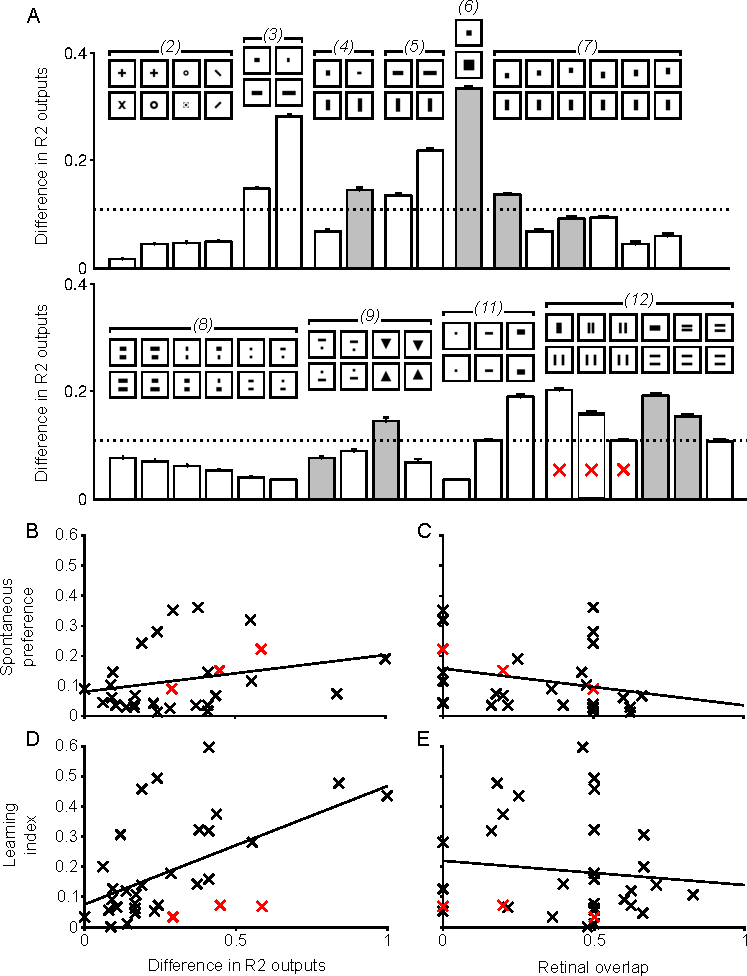
\includegraphics{figures/pattern}
\caption{Outputs of simulated R2 cells for published pattern pairs.
Whether a pattern pair is discriminable by flies can be predicted partly on the basis of the difference in R2 activity.
The patterns tested here are drawn from \protect\cite{Ernst1999} and are grouped together according to the figures in which they appear in that work.
The corresponding figure numbers are shown in parentheses.
All patterns for which the significance of `learning preference' ($\overline{\mathrm{DCP}}$) was given are included.
A: Grey bars indicate that the $\overline{\mathrm{DCP}}$ for the pattern was significant ($p<.05$).
A higher score indicates a greater \ac{rms} difference in R2 activity and thus that the pattern was more discriminable by the simulation.
In general, within these groups, the patterns where there was a significant learned preference have a greater difference in activity \protect\cite{Ernst1999}.
Performance on more `horizontal' patterns (e.g. \emph{(3)} and the final three patterns in \emph{(12)}) was poor in the behavioural experiments, but better in simulation.
This is perhaps due to the horizontal motion of the patterns in training, as noted in \protect\cite{Ernst1999}.
B and C: Scatter plots of R2 difference (the `RF Model') and retinal overlap (the `Retinotopic Model') \emph{vs} spontaneous preference ($\overline{\mathrm{SCP}}$) shown in \protect\cite{Ernst1999}.
No correlation was found for the RF Model (Spearman's rank, $n=29, \rho=.289, p=\mathrm{n.s.}$) or the Retinotopic Model ($n=29, \rho= -0.365, p=\mathrm{n.s.}$).
D and E: Scatter plots of R2 difference (the `RF Model') and retinal overlap (the `Retinotopic Model') \emph{vs} learning index ($\overline{\mathrm{DCP}}$).
A significant correlation was found for the RF Model (Spearman's rank, $n=32, \rho=.501, p < .005$) but not the Retinotopic Model ($n=32, \rho=-.068,p=\mathrm{n.s.}$).
As two of the data points in panel D appeared to be outliers, we reran the analysis excluding these points and found that the correlation was still significant, albeit less so ($n=30, \rho=.420, p < .05$).}
\label{fig:pattern}
\end{figure}

\begin{comment}
==== SCP ====
R2: N = 29; rho = 0.288952; p = 0.128449
ROL: N = 29; rho = -0.364811; p = 0.051678

==== DCP ====
R2: N = 32; rho = 0.501696; p = 0.003440
ROL: N = 32; rho = -0.068018; p = 0.711467

CORRELATION WITHOUT OUTLIERS:
==== DCP ====
R2: N = 30; rho = 0.420514; p = 0.020677
\end{comment}
